\documentclass{beamer}
\usepackage[english]{babel}
\usepackage{calc}
\usepackage[absolute,overlay]{textpos}
\mode<presentation>{\usetheme{tud}}
%\usepackage{subcaption}

\usepackage{tikz}
\usetikzlibrary{decorations.markings}
\usetikzlibrary{shapes,snakes}
\usetikzlibrary{shapes.geometric}
\usetikzlibrary{fit}					
\usetikzlibrary{backgrounds}
\usetikzlibrary{positioning}
\usepackage{pgffor}
\usepackage{amsmath,amssymb}
\usepackage{color}



\usepackage{pifont}
\usepackage{pgfplots}

\tikzstyle{every picture}+=[remember picture]
\tikzstyle{na} = [baseline=-.5ex]


\title[Accuracy of original MPM]{Accuracy of original MPM}
%\institute[]{}
\author[]{Lisa Wobbes, Roel Tielen}
\date[\today]{\today}

\definecolor{blueM}{rgb}{0.4, 0.6, 0.8}

\begin{document}
%titel----------------------------------------------------------------------------------------------------------------------------------------------------------------
{
%\usebackgroundtemplate{\includegraphics[width=\paperwidth,height=\paperheight]{logos}}%
%\setbeamertemplate{footline}{\usebeamertemplate*{minimal footline}}
\frame{\titlepage}
}

%outline------------------------------------------------------------------------------------------------------------------------------------------------------------
\begin{frame}{Outline}
\begin{itemize}
\item Numerical accuracy
\item Benchmarks
	\begin{itemize}
	\item Vibrating linear-elastic bar 
	\item Vibrating hyper-elastic bar
	\item Oedometer
	\end{itemize}
\item
\item
\item
\end{itemize}
\end{frame}

%------------------------------------------------------------------------------------------------------------------
\begin{frame}{Vibrating bar}
\tikzset{
mystyle1/.style={
  rectangle,
  inner sep=0.05pt,
  text width=1mm,
  fill=black
  }
}

\tikzset{
mystyle2/.style={
  circle,
  inner sep=0.1pt,
  text width=2mm,
  fill=red!80
  }
}
\begin{figure}[h]
\centering
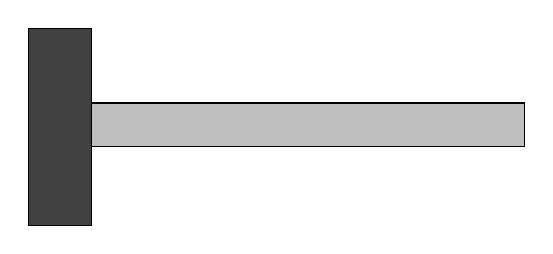
\begin{tikzpicture}
 %structure
 \draw[fill=black!25] (0.5,2) rectangle (6,2.55);
 \draw[fill=black!75] (-0.3,3.5) rectangle (0.5,1);



\end{tikzpicture}
\end{figure}
\end{frame}


%------------------------------------------------------------------------------------------------------------------
\begin{frame}{Oedometer problem}
\definecolor{soil}{cmyk}{0,0.2,0.6,0.2}
\definecolor{darkred}{cmyk}{0,0.9,0.9,0.2}
\tikzset{
mystyle1/.style={
  rectangle,
  inner sep=0.05pt,
  text width=1mm,
  fill=black
  }
}

\tikzset{
mystyle2/.style={
  circle,
  inner sep=0.1pt,
  text width=2mm,
  fill=red!80
  }
}
\begin{figure}[h]
\centering
\begin{tikzpicture}
 %structure
 \draw[fill=black] (0.4,2.2) rectangle (2.6,-1.1);
 \draw[fill=soil] (0.5,2) rectangle (2.5,-1);
 \draw[fill=black!25] (0.5,2) rectangle (2.5,2.35);
 \draw (1.5, 0.5) node {soil};
 %coordinates
 \draw (3.2,2) node {$y$ = 1};
 \draw (3.2,-1) node {$y$ = 0};
 %load
 \draw[->, ultra thick,darkred] (0.7,3) -- (0.7,2.35);
 \draw[->, ultra thick,darkred] (1.5,3) -- (1.5,2.35);
 \draw[->, ultra thick,darkred] (2.3,3) -- (2.3,2.35);
 \draw (1.55,3.3) node {$p_0$};
%coordinate
\draw[->, thick] (-1,-1)--(-1,0);
\draw (-1, 0.3) node {$y$};

\draw (1.7,-2) node {schematic representation};

\end{tikzpicture}
\end{figure}
\end{frame}

%------------------------------------------------------------------------------------------------------------------
\begin{frame}{Oedometer: model}
\begin{align}\nonumber
 &\rho \frac{\partial \hat{v}}{\partial t} = \frac{\partial \hat{\sigma}}{\partial y} - \rho g, \\ \nonumber
 &\frac{\partial \hat{\sigma}}{\partial t} = E \frac{\partial \varepsilon}{\partial t}.
\end{align}
Boundary conditions: 
\begin{align} \nonumber
 &\hat{v}(0,t)  = 0,\\ \nonumber
 &\hat{\sigma}(H,t)  = -p_0.
\end{align}
Initial conditions:
\begin{align} \nonumber
 \hat{v}(y,0)&=0,\\ \nonumber
 \hat{\sigma}(y,0)&=0.
\end{align}
\end{frame}








\end{document}
\grid
